
%(BEGIN_QUESTION)
% Copyright 2006, Tony R. Kuphaldt, released under the Creative Commons Attribution License (v 1.0)
% This means you may do almost anything with this work of mine, so long as you give me proper credit

Suppose someone were to connect a precision potentiometer to a temperature instrument using thermocouple wire, except that they chose the wrong type of thermocouple wire:

$$\includegraphics[width=15.5cm]{i00423x01.eps}$$

The instrument technician performing the calibration sets the potentiometer to an output of 20.871 millivolts, hoping to simulate a temperature of 1000$^{o}$ F for the temperature instrument to measure.  However, since the wrong type of thermocouple wire is being used (type S instead of type K), the instrument will actually register something else.

Assuming the instrument is already properly calibrated, what temperature will it indicate with a potentiometer output of 20.871 mV and the indicated ambient temperatures?

\underbar{file i00423}
%(END_QUESTION)





%(BEGIN_ANSWER)

The instrument will register 993.5$^{o}$ F.

%(END_ANSWER)





%(BEGIN_NOTES)


%INDEX% Measurement, temperature: thermocouple

%(END_NOTES)


